\section{Results and Discussion}

The longitudinal and transversal spatial wave function densities for $\eta = 10 \, \omega_\text{r}$ are depicted in Figure~\ref{densities}. The leftmost state is the first eigenstate, the second eigenstate is in the middle and the third on the right. Both for longitudinal and transversal pump, because of equal contributions of $a$ and $a^\dagger$, the spatial densities are $\lambda / 2$-periodic. The first eigenstate has the lowest energy. Each peak of the ground state density being located at the potential minima is in accordance with our expectations. However, these graphs don't give us enough insight into the physical processes of the system. For that purpose, looking at the momentum space is more fruitful.

\begin{figure}[!htb]
	\begin{minipage}[b]{1\linewidth}
	\centering
	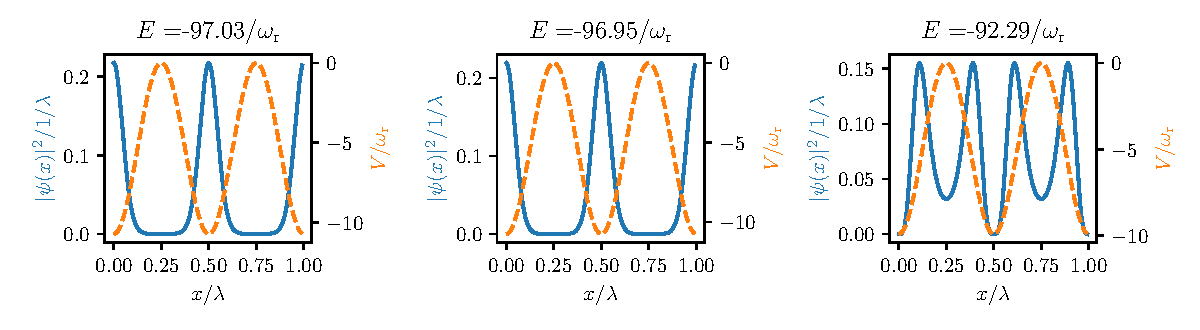
\includegraphics[width=1\textwidth]{images/dens_long.pdf}
	\subcaption{Longitudinal.}
	\label{long_density}
	\end{minipage}
%
	\begin{minipage}[b]{1\linewidth}
	\centering
	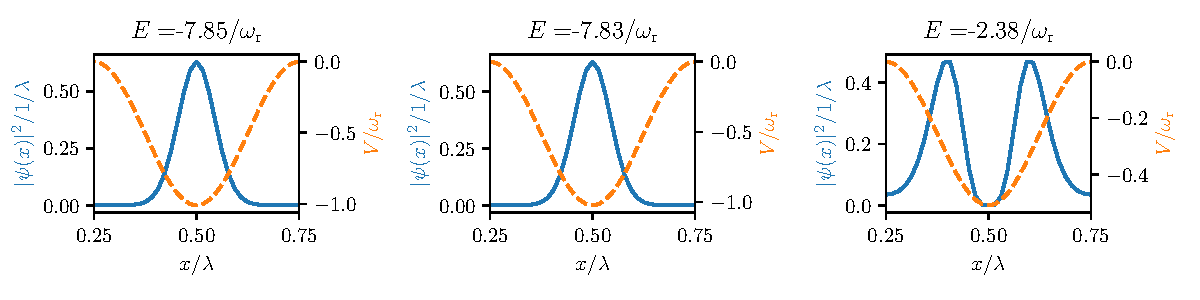
\includegraphics[width=1\textwidth]{images/dens_trans.pdf}
	\subcaption{Transversal.}
	\label{trans_density}
	\end{minipage}
\caption{Longitudinal and transversal wave function densities for $\eta = 10 \, \omega_\text{r}$. The first eigenstate is on the left, the second in the middle and the third on the right. The wave function densities being located at potential minima meets our expectation, however much of the physics of the system remains hidden to us in this plot. The momentum plot gives us more insight.}
\label{densities}
\end{figure}
\FloatBarrier

\noindent The momentum distribution for different values of $\eta$ can be seen in Figure~\ref{momenta}. Here we can see much more of the actual physics of the system. At $\eta = 0$, i.e. when the laser is off, there's only a peak at 0, meaning the atoms have no momentum. When we start pumping, we get other peaks than 0. Now the atoms do have momentum. For longitudinal pumping, there's always a gap between each peak, which is not the case for transversal pumping. Take a look again at figure~\ref{pumping}. When we pump longitudinally, a photon is only able to transfer a momentum of $2 \hbar k$ because of momentum conservation. Thus we only observe peaks at $2n\hbar k$, where $n \in \mathbb{N}$. For transversal pumping, the same processes of photons transferring momenta of $2\hbar k$ are happening, but now we also have a momentum transfer of $\hbar k$ when a transversally incoming photon is being scattered into the cavity. Naturally, the more we pump, the more outer momenta we will get.

\begin{figure}[!htb]
	\begin{minipage}[b]{1\linewidth}
	\centering
	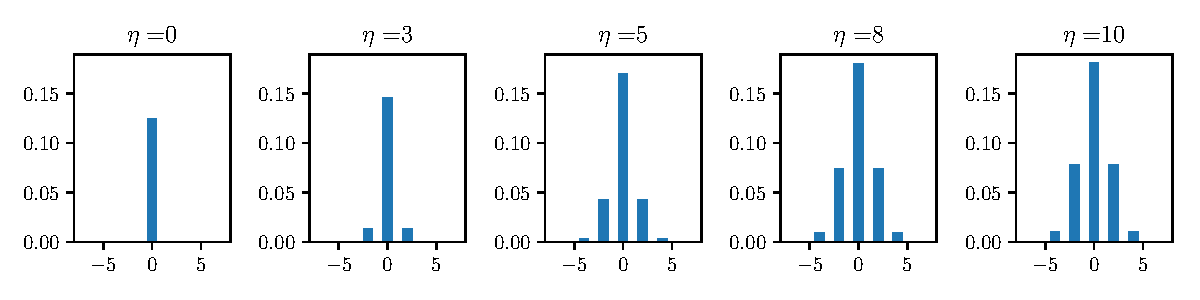
\includegraphics[width=1\textwidth]{images/mom_long.pdf}
	\subcaption{Longitudinal.}
	\label{long_momentum}
	\end{minipage}
%
	\begin{minipage}[b]{1\linewidth}
	\centering
	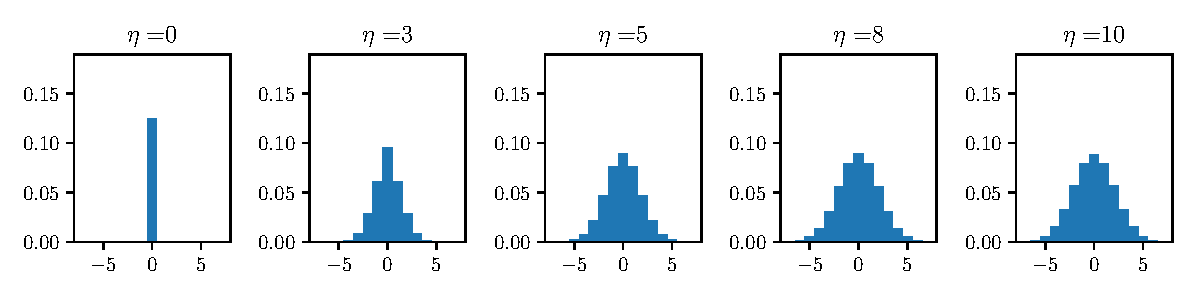
\includegraphics[width=1\textwidth]{images/mom_trans.pdf}
	\subcaption{Transversal.}
	\label{trans_momentum}
	\end{minipage}
\caption{Longitudinal and transversal momentum distributions. For longitudinal pump, there are only momenta of $2 n \hbar k$ because longitudinal scattering processes only allow momenta transfer of $2 \hbar k$. For transversal pump, there is no such restriction and we have momenta of $n \hbar k$.}
\label{momenta}
\end{figure}
\FloatBarrier

\noindent Having looked at the atom part of the composite system, let's take a look at the photon part. The photon number distribution for different values of $\eta$ can be seen in Figure~\ref{photon_dist}. The mean and variance are pretty much the same, thus we have a Poisson distribution.

\begin{figure}[!htb]
	\begin{minipage}[b]{1\linewidth}
	\centering
	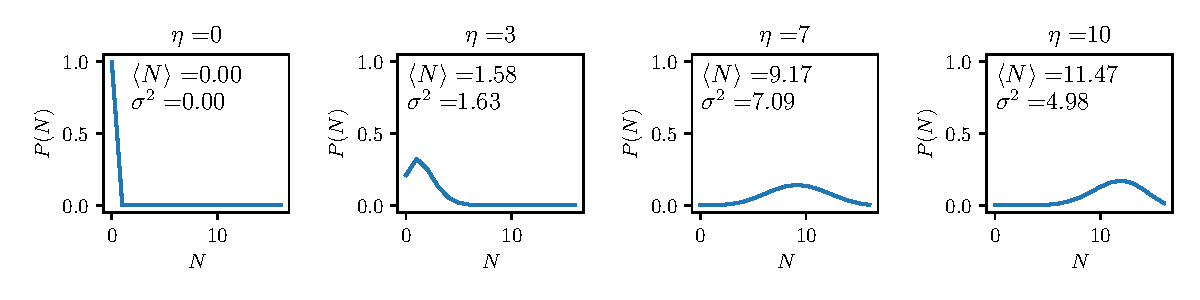
\includegraphics[width=1\textwidth]{images/pho_dens_long.pdf}
	\subcaption{Longitudinal.}
	\end{minipage}
%
	\begin{minipage}[b]{1\linewidth}
	\centering
	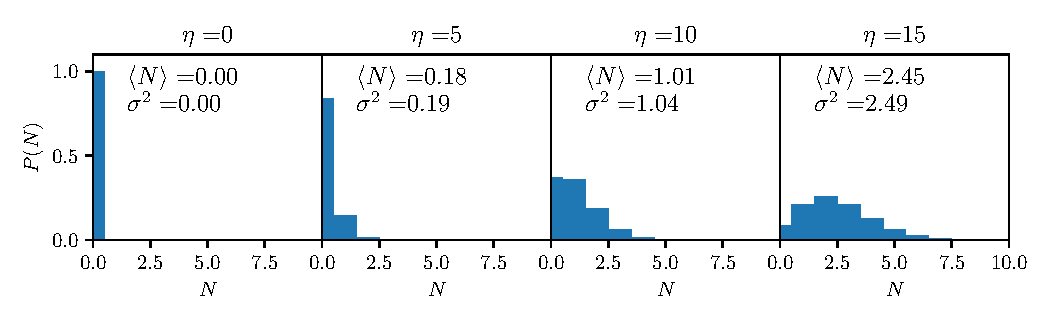
\includegraphics[width=1\textwidth]{images/pho_dens_trans.pdf}
	\subcaption{Transversal.}
	\end{minipage}
\caption{Longitudinal and transversal photon distributions. Since the mean and the variance are the same, we have a Poisson distribution.}
\label{photon_dist}
\end{figure}
\FloatBarrier

\noindent The Husimi Q representation of the photon states of both longitudinal and transversal pump can be seen in Figure~\ref{qfunc}. We remind ourselves that the $x$-axis represents the position while the $y$-axis represents the momentum of the state. To each state there's a quantum uncertainty of $1/2$, thus we don't see a point but a blob. At $\eta = 0$, there's no momentum since we don't pump at all and the blob is in the center. For longitudinal pumping, increasing $\eta$ will directly result in more photon momentum and the blob rises. That's not the case for transversal pumping. Initially, increasing $\eta$ will only result in more momentum uncertainty, hence the blob stretches. At a sufficient pump strength, the blob will separate into two. Two blobs means we're actually looking at the superposition of two states that are symmetric. Before the separation, the highest probability of the momentum is still at 0 meaning that when we pump transversally, the light field initially resists self-ordering.


\begin{figure}[!htb]
	\begin{minipage}[b]{1\linewidth}
	\centering
	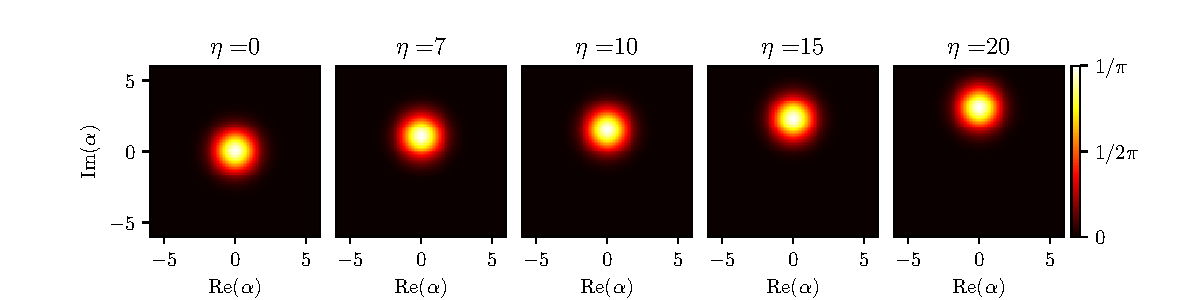
\includegraphics[width=1\textwidth]{images/qfunc_long.pdf}
	\subcaption{Longitudinal.}
	\end{minipage}
%
	\begin{minipage}[b]{1\linewidth}
	\centering
	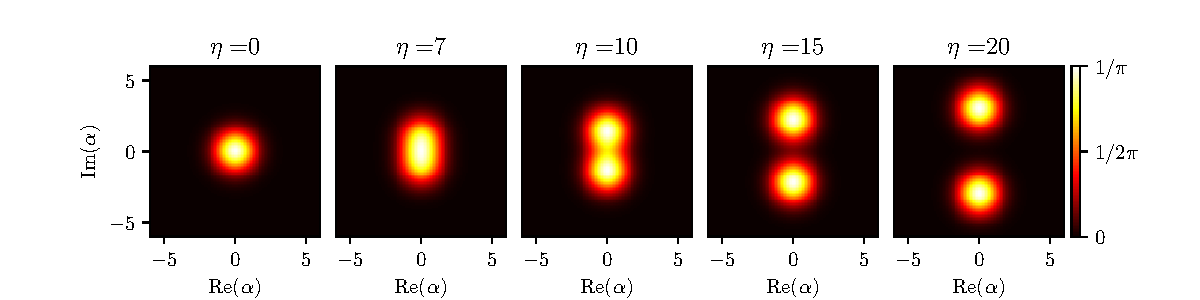
\includegraphics[width=1\textwidth]{images/qfunc_trans.pdf}
	\subcaption{Transversal.}
	\end{minipage}
\caption{Husimi Q representation of photon states for longitudinal and transversal pumping. The $y$-axis represents the momentum of the state. For longitudinal pumping, increasing $\eta$ directly results in more momentum. For transversal pumping, the state initially resists and the mean of the momentum stays at 0. Only at sufficient pump strengths, the momentum will rise which indicates self-ordering of the system. Observing two blobs for transversal pumping means we're actually looking at the superposition of two symmetric states.}
\label{qfunc}
\end{figure}
\FloatBarrier

\noindent If we were to measure the system experimentally, we'd only obtain one blob since measuring means breaking the symmetry. The superposition is also reflected in the fact that the graph of Figure~\ref{densities} with transversal pumping is $\lambda / 2$-periodic. Actually, it should be $\lambda$-periodic. Figure~\ref{densities_superposition} illustrates the superposition and the lattice of the atoms.

\begin{figure}[!htb]
	\begin{minipage}[b]{.5\linewidth}
	\centering
	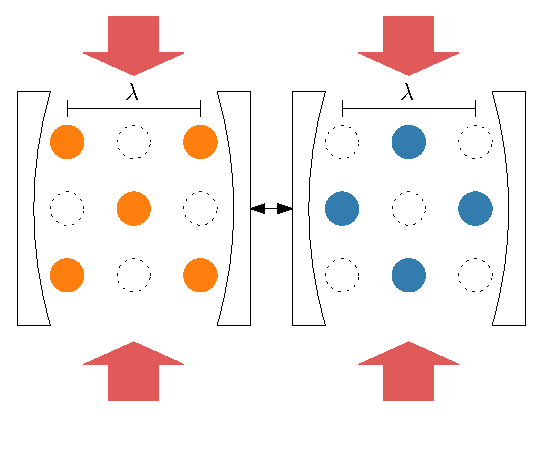
\includegraphics[width=.9\textwidth]{images/lattice_drawing.eps}
	\subcaption{Lattice.}
	\end{minipage}
%
	\begin{minipage}[b]{.5\linewidth}
	\centering
	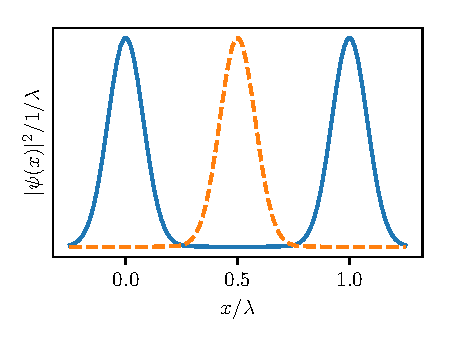
\includegraphics[width=.9\textwidth]{images/density_superposition.pdf}
	\subcaption{Densities.}
	\end{minipage}
\caption{Lattice configuration and superposition of densities. If we were to measure the system experimentally, we'd only obtain one lattice pattern. In this simulation, however, we obtain the two configurations simultaneously, thus observing a $\lambda/2$-periodic wave function density.}
\label{densities_superposition}
\end{figure}
\FloatBarrier

\noindent We can break the symmetry artificially by only looking at one half of the graph. Figure~\ref{fig_order_param} shows the momentum with the highest probability for longitudinal and transversal pumping. For longitudinal pumping, the momentum increases linearly. The light field gets stronger and stronger and the atoms will order gradually. For transversal pumping, the light field initially does not acquire any momentum which means that the atoms are resisting ordering. At a critical pump strength, we see that the momentum suddenly increases very rapidly and self-ordering of the atoms takes place.

\begin{figure}[!htb]
	\begin{minipage}[b]{.5\linewidth}
	\centering
	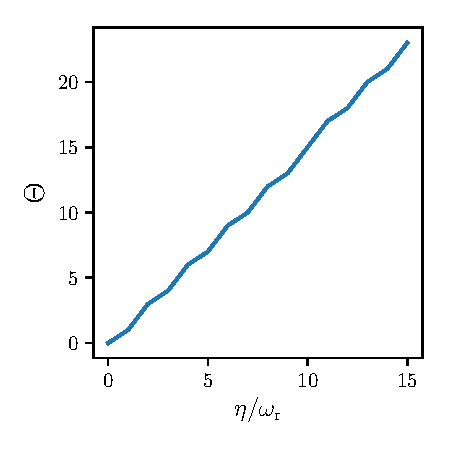
\includegraphics[width=.9\textwidth]{images/theta_long.pdf}
	\subcaption{Longitudinal.}
	\end{minipage}
%
	\begin{minipage}[b]{.5\linewidth}
	\centering
	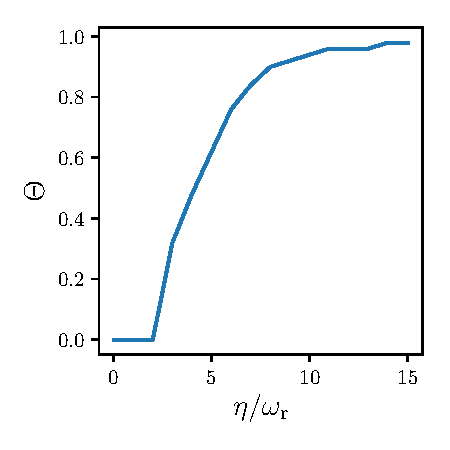
\includegraphics[width=.9\textwidth]{images/theta_trans.pdf}
	\subcaption{Transversal.}
	\end{minipage}
\caption{Most likely value of the photon state momentum looking at only the positive side of the phase space for longitudinal and transversal pumping. For longitudinal pumping, the momentum increases gradually. For transversal pumping, the light initially does not gain any momentum, meaning that the atoms resist being in order. At a critical pump strength, a light field suddenly builds up and the atoms self-order.}
\label{fig_order_param}
\end{figure}
\FloatBarrier

\noindent The more we pump, the more photons will appear. We have to take that into account by raising the maximum amount of allowed photon states $N_\text{cutoff}$. Raising $N_\text{cutoff}$ results in longer simulation times, however if we don't do so, our results become faulty. Take a look at Figure~\ref{model_limit} which depicts the photon number distributions for different values of $N_\text{cutoff}$ at $\eta = 40 \, \omega_\text{r}$. For our parameters, $40 \, \omega_\text{r}$ is a relatively high value for $\eta$ and we thus would expect a high average photon number which cannot be the case if limit $N_\text{cutoff}$ to 8. To check the validity of our results, i.e. if $N_\text{cutoff}$ is set high enough, we can look at the standard deviation. For a Poisson distribution, the mean has to be the same as the standard deviation which is not the case if we set the cutoff too low.

\begin{figure}[!htb]
	\centering
	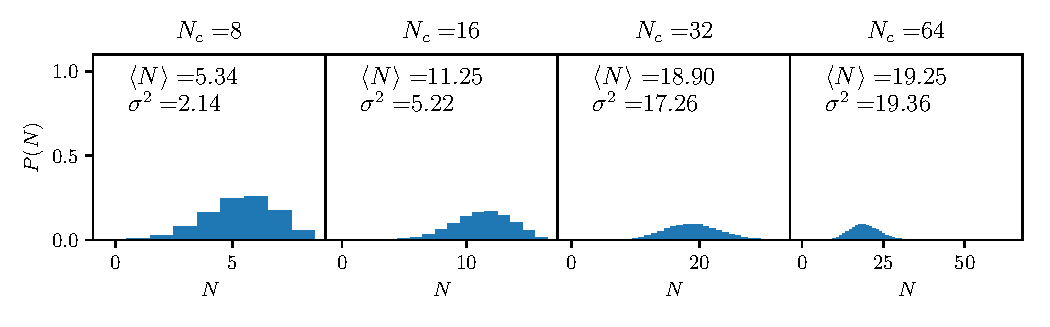
\includegraphics[width=1\textwidth]{images/model_limit_long.pdf}
	\caption{Photon number distributions for different values of $N_\text{cutoff}$ at $\eta = 40 \, \omega_\text{r}$. If we don't set $N_\text{cutoff}$ sufficiently high, we get bogus results. A quick sanity check is to compare the mean with the variance. For a Poisson distribution, they have to be the same.}
	\label{model_limit}
\end{figure}
\FloatBarrier
